
%%
\newcommand{\cg}[1]{\cellcolor{green!25}#1}
\newcommand{\ce}[1]{\cellcolor{red!25}#1}
\newcommand{\cb}[1]{\cellcolor{gray!25}#1}
\newcommand{\n}{n/a}
\newcommand{\citeP}{\cite{Petersen2013}}
\newcommand{\citeCs}{\cite{Chelton2007}}
\newcommand{\citeCe}{\cite{Chelton2011}}
\newcommand{\citeCes}{\cite{Chelton2011,Chelton2007}}
\begin{frame}
 \frametitle{to-do-matrix}
 \begin{small} 
\begin{tabular}{r|c|c|c|}
\multicolumn{1}{c}{}	& \multicolumn{1}{c}{pop}	&	\multicolumn{1}{c}{aviso}	&	\multicolumn{1}{c}{comparison}\\
\cline{2-4}
U						&	\cg{\citeP}				&		\cg{\citeCes}			&		\cg{\citeP}	\\
\cline{2-4}
scale					&	\cg{\citeP}				&		\cg{\citeCes}			&		\cg{\citeP}	\\
\cline{2-4}
method Chelton			&	\ce{N}					&		\cg{\citeCe,N}			&		\ce{N}	\\
\cline{2-4}
method $R^2$			&	\cg{\citeP}				&		\cb{\n}					&		\cb{\n}	\\
\cline{2-4}
method OW				&	\cg{\citeP}				&		\cg{\citeCs}			&		\cg{\citeP}	\\
\cline{2-4}
method IQ				&	\ce{N}					&		\ce{N}					&		\ce{N}	\\
\cline{2-4}
net U					&	\ce{N}					&		\ce{N}					&		\ce{N}	\\
\cline{2-4}
steering level			&	\ce{N}					&		\cb{\n}					&		\cb{\n}	\\
\cline{2-4}
$p(z)$					&	\ce{N}					&		\cb{\n}					&		\cb{\n}	\\
\cline{2-4}
$f/H$					&	\ce{N}					&		\ce{ }					&		\ce{ }	\\
\cline{2-4}
remap pop2avi
&	\ce{ }					&		\ce{ }					&		\ce{ }	\\
\cline{2-4}
drop buoys into eddies
&	\ce{ }					&		\ce{ }					&		\ce{ }	\\
\cline{2-4}
go 3d
&	\ce{ }					&		\ce{ }					&		\ce{ }	\\
\cline{2-4}
\end{tabular}
\end{small}
\begin{tiny}
\bibliographystyle{acm}
\bibliography{/home/niko/documents/library}
%\bibliography{/home/zmaw/u300065/mendeley/library}
\end{tiny}
\end{frame}


%\begin{frame}
%\bibliographystyle{acm}
%\bibliography{/home/zmaw/u300065/mendeley/library}
%\bibliography{/home/niko/documents/library}
%\end{frame}


\begin{frame}
\frametitle{Which depth to take mean current from?}
\begin{figure}
	\centering
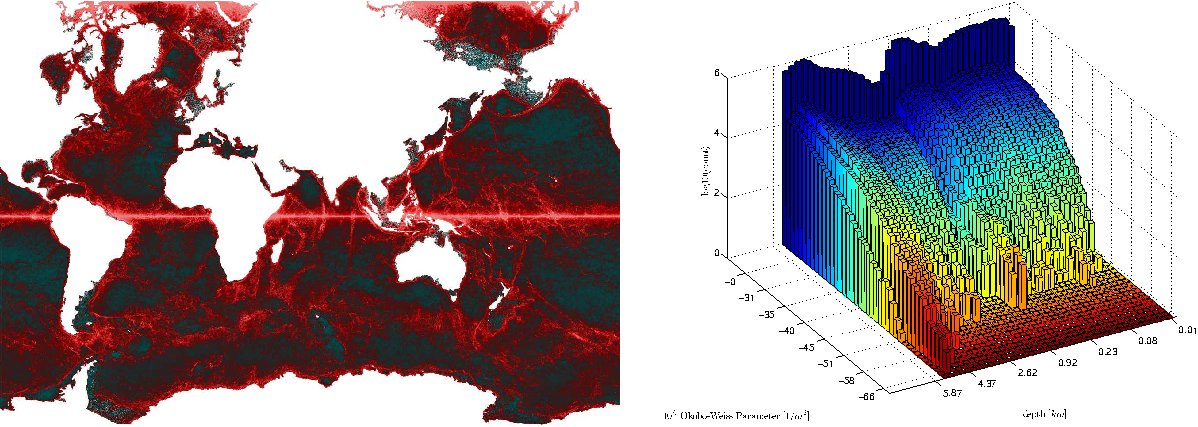
\includegraphics[width=330pt,keepaspectratio=true]{OWdouble.pdf}
\end{figure}
\end{frame}






